\documentclass{article}
\usepackage[slovak]{babel}
\usepackage[T1]{fontenc}
\usepackage[utf8]{inputenc}
\usepackage[a4paper, left=2.5cm, right=2.5cm, top=2.5cm, bottom=2.5cm]{geometry}
\usepackage{changepage}
\usepackage{microtype}

\usepackage[
	backend=biber
	,style=iso-numeric
	,language=czech
	,autolang=other
	,sortlocale=sk_SK
]{biblatex}

\usepackage[texindy,nonewpage]{imakeidx}
\makeatletter
\def\imki@putindex#1{%
	\ifimki@nonewpage\else
	\imki@clearpage
	%% The following two lines are incorrectly switched in the package:
	\immediate\closeout\csname #1@idxfile\endcsname
	\fi
	\let\imki@indexname\indexname % keep \indexname
	\@nameuse{imki@set@#1}\imki@decide
	\if@tempswa % we can call the external program
	\imki@exec{\imki@program\imki@options#1.idx}%
	\else
	\imki@finalmessage{#1}%
	\fi
	\ifKV@imki@intoc
	\def\imki@maybeaddtotoc{\@nameuse{phantomsection}%
		\addcontentsline{toc}{\imki@toclevel}{\imki@title}}%
	\else
	\def\imki@maybeaddtotoc{}%
	\fi
	\ifx\imki@title\imki@check@indexname\else
	\def\indexname{\imki@title}%
	\fi
	\@input@{#1.ind}
	\let\indexname\imki@indexname % restore \indexname
}
\makeatother

\usepackage{graphicx}

\usepackage[unicode]{hyperref}

\languageattribute{slovak}{split}

\setlength{\parindent}{1,25cm}

\bibliography{references.bib}

\makeindex[
	title=Register
	,options=
		-I omega
		--language slovak
]
% Koniec preambuly.

\begin{document}
\begin{center}
\Huge
\textbf{\textit{Životopis}}
\end{center}
\bigskip

\begin{flushleft}
\Large
\textit{\textsf{Kontaktné údaje}}
\normalsize

\smallskip

Richard Kalinec

+421 xxx xxx xxx

yyyyyyyyyyy@zzzzzzz.zzz
\end{flushleft}

\bigskip

\begin{flushleft}
\Large
\textit{\textsf{Osobné údaje}}
\normalsize
\end{flushleft}

\smallskip

\begin{adjustwidth}{-6pt}{}
\begin{tabular}{l l}
	Adresa: & Ulica xx, 962 12 Detva \\
	Dátum narodenia: & xx.xx.1993
\end{tabular}
\end{adjustwidth}

\bigskip

\begin{flushleft}
\Large
\textit{\textsf{Vzdelanie}}
\normalsize
\end{flushleft}

\smallskip

\begin{adjustwidth}{-6pt}{}
\begin{tabular}{l l}
	1999 - 2008: & 4. Základná škola/Základná škola Júliusa Juraja Thurzu v~Detve\\
	2008 - 2012: & Gymnázium v~Detve\\
	2012 - súčasnosť: & Fakulta informatiky Masarykovej univerzity v~Brne\\
\end{tabular}
\end{adjustwidth}

\bigskip

\begin{flushleft}
\Large
\textit{\textsf{Jazykové znalosti}}
\normalsize
\end{flushleft}

\smallskip

\begin{adjustwidth}{-6pt}{}
\begin{tabular}{l l}
Anglický jazyk: & aktívne slovom aj písmom \\
Nemecký jazyk: & začiatočník
\end{tabular}
\end{adjustwidth}

\bigskip

\begin{flushleft}
\Large
\textit{\textsf{Počítačové znalosti - Používateľ}}
\normalsize
\end{flushleft}

\smallskip

\begin{adjustwidth}{-6pt}{}
	\begin{tabular}{l l}
		Microsoft Word, Excel a~PowerPoint: & denný používateľ \\
		Správa MS Windows: & pokročilý \\
		Správa Ubuntu a~Fedory: & začiatočník \\
		Programovanie v~C, C++ a~C\#: & pokročilý \\
		Programovanie v~Jave: & začiatočník
	\end{tabular}
\end{adjustwidth}

\bigskip

\begin{flushleft}
\Large
\textit{\textsf{Ďalšie znalosti, schopnosti a~záujmy}}
\normalsize
\end{flushleft}

\smallskip

\begin{flushleft}
\large
Vlastnosti:
\end{flushleft}

Považujem sa za zodpovedného a~ochotného človeka, na ktorého sa dá spoľahnúť. Najlepšie zvládam rutinné a~mechanické činnosti, ktoré mnohých iných ľudí nudia, taktiež som však celkom dobrým tímovým hráčom. Som preto presvedčený, že by som mohol pracovný kolektív v~mnohom pozitívne dopĺňať. Rovnako verím, že budem schopný pozitívne prispieť k~atmosfére na pracovisku najmä prívetivosťou a~psychickou podporou.

\smallskip

\begin{flushleft}
\large
Záujmy:
\end{flushleft}

Zaujímam sa o~domáce aj svetové dianie najmä v~politike a~ekonomike,
ale aj o~históriu a~psychológiu. Rád filozofujem a~na mnohé veci sa
pozerám z~netypických uhlov pohľadu. Taktiež veľa rozmýšľam, ako robiť veci lepšie, som perfekcionista, ktorý sa ale čoraz viac pragmaticky krotí, keď je to vhodné.

\bigskip

\texttt{Richard Kalinec, 12.11.2015, Brno}

\pagebreak

\begin{center}
\Huge
\textbf{\textit{Monitorovanie, analýza a~uchovávanie elektronickej komunikácie tajnými službami}}
\normalsize
\end{center}

\bigskip

Uplynulý rok ostala široká verejnosť na celom svete šokovaná odhalením, že jedna z~tajných služieb USA, National Security Agency (NSA)\index{NSA} \cite{nsa}, ale aj jedna z~tajných služieb Veľkej Británie, Government Communications Headquarters (GCHQ)\index{GCHQ} \cite{gchq}, zhromažďujú, vyhodnocujú a~ukladajú údaje o~elektronickej komunikácii na celom svete. Bývalý technik amerických tajných služieb Edward Snowden\index{Edward Snowden}, ktorý tieto skutočnosti poskytol viacerým svetoznámym médiám, radšej utiekol do Ruska. \cite{techsme1,sme1} Zo strany prevažnej časti odbornej aj laickej verejnosti sa začala ozývať ostrá kritika\index{kritika} bezprecedentného zásahu do súkromia\index{súkromie} nevinných ľudí, americká vláda sa aspoň navonok obhajuje, že jej tieto špionážne programy pomáhajú zaistiť bezpečnosť\index{bezpečnosť}. Či americká vláda hovorí pravdu, môžeme len špekulovať, prípadne veriť naším dojmom. Je jasné, že údaje získané špionážou takého rozsahu sú obzvlášť pomocou sofistikovaných analytických nástrojov (hoci sú ich možnosti stále výrazne obmedzené) zneužiteľné\index{zneužitie} hrozivým spôsobom.

\begin{center}
***
\end{center}

Takže tu máme najvyspelejšie sledovacie programy v~dejinách ľudstva, ktoré sú obhajované imperatívom ochrany a~bezpečnosti nevinných ľudí, ako aj tradičného presadzovania národných záujmov a~na druhej strane oprávnene kritizované\index{kritika} nielen za všadeprítomné zásahy do súkromia\index{súkromie}, ale aj za otáznu účinnosť v~praxi.

\smallskip

V~prvom rade som presvedčený, že tajné služby takýmto sledovaním už zašli priďaleko a~nemajú právo takto zasahovať ľuďom do súkromia\index{súkromie}. Ochrana ľudí aj inštitúcií je legitímny záujem, ale ako raz povedala jedna Američanka „Ak stratíme slobodu, stratíme všetko.“. Strach bol a~je mocnými zneužívaný na manipuláciu a~podrobovanie si ľudí. Takáto špionáž porušuje právo ľudí na súkromie a~dáva vláde aj zamestnancom tajnej služby priestor na zneužitie týchto informácií na rôzne nekalé ciele. Áno, vláda to môže myslieť dobre, ale všetko má svoje hranice. Zvlášť v~tajnej službe, ktorá de facto „kontroluje“\index{kontrola} samu seba, keďže aj kontrolné orgány a~príslušný súd sa musia spoľahnúť na to, že tajná služba im hovorí pravdu a~dodržiava zákony, je veľký priestor aj pre zneužitie jednotlivcami pre osobné ciele. Šéfredaktor Guardianu\index{Guardian} – britského denníka, ktorý materiály od Snowdena zverejňuje a~stal sa za to terčom nátlaku britských tajných služieb aj politikov – to vystihol: „Za posledné tri roky sa stalo už po druhýkrát, keď veľmi mladý pracovník na nízkom stupni vedel prečítať ich dáta a~odísť s~nimi. Myslím, že by bolo lepšie, keby sa starali viac o~vlastné zabezpečenie siete ako Guardian.“. Špionáž preto treba aspoň obmedziť a~nájsť spôsob, ako činnosť služby čo najúčinnejšie nezávisle a~transparentne kontrolovať\index{kontrola}. Žiadny kontrolný mechanizmus ale nie je dokonalý, ľudia sú omylní, manipulovateľní a~žiaľ, niektorí aj podplatiteľní či vydierateľní. Takže jedinou spoľahlivou ochranou súkromia ľudí je obmedzenie špionáže. Nedá sa zneužiť\index{zneužitie} údaje, ktoré neboli zachytené...

\begin{center}
	***
\end{center}

Fakt, že aj iné krajiny by radi vykonávali takúto sofistikovanú špionáž, ak by to dokázali, že nedemokratické krajiny sa dopúšťajú ešte horších „opatrení“ voči občanom a~zo súčasného zhrozenia z~americkej a~britskej špionáže sa môžu smiať, neospravedlňuje to, že takúto špionáž vykonávajú USA, Veľká Británia ani nikto iný. Už deťom sa hovorí: „To, že on skočí do studne, neznamená, že máš aj ty.“. Škoda, že sa toho nedržia mnohí dospelí a~v~tomto prípade dokonca tí, ktorí majú na zákonnosť (a~teda aj morálku) v~spoločnosti dohliadať. Áno, na druhej strane vo vzťahu k~zločincom a~nedemokratickým krajinám s~neskrývanými mocenskými ambíciami sa nemôžeme správať vo všetkých ohľadoch tak, ako k~vlastným bezúhonným občanom, ktorí si chcú primerane užiť svoje slobody. Lenže medzi potrebnou až nutnou sebaobranou a~prispôsobením sa nepriaznivej realite na strane jednej a~morálnym relativizmom a~robením tých istých zlých vecí (akurát v~menšom rozsahu a~krajšom kabáte) je nebezpečne tenká a~neostrá hranica. Tým sa vraciame k~citátu spomenutému na začiatku úvahy. Ak chceme byť lepší, musíme počítať s~tým, že to budeme mať zložitejšie a~náročnejšie. Nemôžeme sa nechať prevalcovať zlom, ale ak by bolo bytie dobrým vždy jednoduché a~ľahké, azda by zla ani nebolo... tak sa odpútajme od vyhovárania sa na druhých a~pokúsme sa nájsť cestu, ako sa dá bezpečnosť zaistiť bez neobmedzených praktík „Veľkého brata“. Aj sám Snowden pôvodne utajovanie informácií schvaľoval a~ľudí, ktorí vynášajú informácie, ostro odsudzoval. \cite{techsme3} Nakoniec ale tvárou v~tvár praktikám v~tajnej službe zmenil názor... Novinár spolupracujúci s~ním tvrdí, že „má dosť informácií, ktoré by Spojeným štátom narobili za minútu viac škody, ako sa podarilo komukoľvek inému v~histórii USA... Lenže to nie je jeho cieľ.“. \cite{sme3} Aj šéfredaktor Guardianu nedávno vyhlásil, že zverejnili iba jedno percento materiálov, „urobili veľmi selektívne\index{selekcia} úsudky“ o~tom, čo zverejniť a~neodhalil žiadne meno zamestnanca tajnej služby. \cite{sme2}

\begin{center}
	***
\end{center}

Špionáž\index{špionáž} takéhoto rozsahu je teda neprijateľná bez ohľadu na to, kto by to tiež rád robil či kto robí ešte horšie veci. Mantra bezpečnosti\index{bezpečnosť} či národných záujmov\index{národné záujmy} bola v~histórii nespočet krát zneužitá v~mocenskom boji\index{mocenský boj}, ako aj na presadzovanie autoritárskych a~slobody\index{sloboda} potláčajúcich politík. A~ak aj sú tieto snahy myslené úprimne dobre, napriek vidine potenciálnych bezpečnostných prínosov je nutné nebagatelizovať hrozivé riziká zneužívania\index{zneužitie} plošne zhromažďovaných údajov.

Hoci je teda problematika špionáže rozporuplná, vlády USA a~Veľkej Británie by mali urobiť všetko pre to, aby našli adekvátny spôsob sledovania komunikácie, ktorý bude čo najlepšie vyvažovať prínos pre bezpečnosť\index{bezpečnosť} a~elimináciu rôznych hrozieb na strane jednej a~rešpektovanie súkromia\index{súkromie} ľudí, ako aj obmedzenie možností zneužitia\index{zneužitie} vládou aj pracovníkmi tajných služieb na strane druhej. Ich dôveryhodnosti môže čo najúčinnejšia nezávislá a~transparentná kontrola\index{kontrola} sledovacích programov, ktoré by plnili práve ten účel, pre ktorý boli oficiálne zriadené, len prospieť. Takisto by nehnali vodu na mlyn úvahám o~rozštiepení internetu a~pokusom o~vytváranie uzavretých národných sietí.

Bude teda veľmi zaujímavé sledovať, ako sa vyvinie do veľkej miery hodnotový boj medzi súkromím\index{súkromie}, ale aj slobodou\index{sloboda} na jednej strane, a~pocitom istoty a~bezpečnosťou\index{bezpečnosť} na druhej strane. Samozrejme, zásadnú úlohu zohrajú analýzy a~diskusie okolo praktických poznatkov a~vízií. Avšak rozhodnutie v~tomto prípade zrejme nastaví dôležitý precedens aj pre iné oblasti života. Je to skúška, kam až sme odhodlaní posúvať našu slobodu\index{sloboda} a~dôveru v~schopnosť ľudstva morálne dospieť natoľko, že nebude potrebovať, aby štáty boli príliš veľké, silné a~nedôverčivé, aby sme si z~našej civilizácie neurobili džungľu. A~tiež skúška, či sa nakoniec väčšina uspokojí s~tým, že v~náručí „Veľkého brata“ je život aspoň na prvý pohľad predsa len pohodlnejší a~istejší. Aj za cenu neduhov v~štátnej správe či dokonca diktatúre, ktoré by bohato vystačili azda na nejednu ďalšiu esej...

\begin{figure}[htbp]
\begin{center}
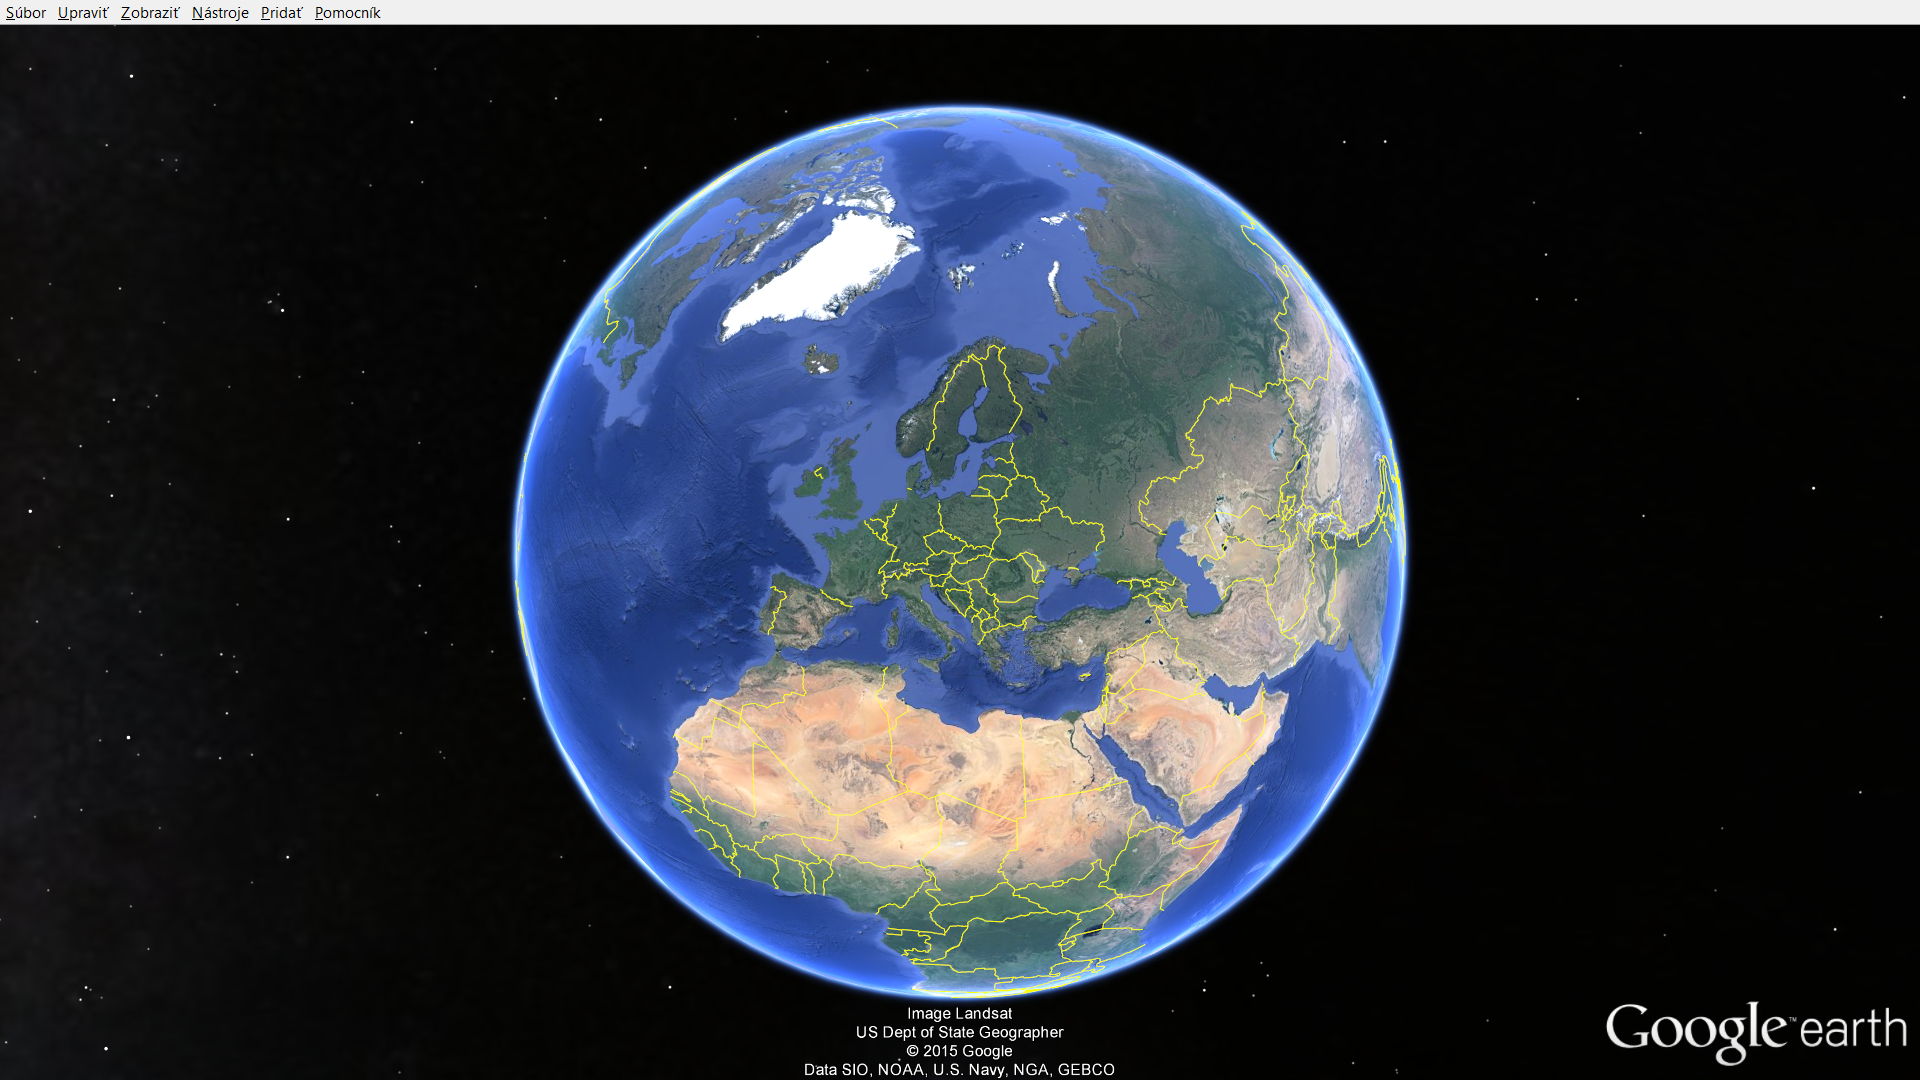
\includegraphics[width=\textwidth]{Zem_2015-9-17}
\end{center}
\end{figure}

\nocite{cnn1}
\nocite{techsme2}
\nocite{techidnes2}
\nocite{sme4}
\nocite{sme8}

\printbibliography

\printindex

\end{document}